\chapter{绪论}
\label{cha:introduction}
\section{选题背景与意义}

360°视频流内容允许用户在观看视频时在多个方向上改变她/他的观看方向,从而获得比观看具有固定观看方向的传统视频内容更身临其境的体验。此类视频内容可以使用不同的设备观看,从智能手机和台式电脑到特殊的头戴式显示器 (HMD),如 Oculus Rift、三星 Gear VR、HTC Vive 等。使用 HMD(Human Mounted Display) 观看此类内容时,可以通过头部移动来改变观察方向。在智能手机和平板电脑上,可以通过触摸交互或通过内置传感器移动设备来改变观看方向。在台式电脑上,鼠标或键盘可用于与全向视频交互。360°视频流能够提供全景视图,让用户拥有身临其境的体验,现在在主要的视频共享网站和社交媒体渠道上越来越流行。近些年来,随着“元宇宙”等概念越来越热门以及头戴式设备的深入研究使得价格不断下降,“虚拟现实”也越来越热门。“虚拟现实”中也有相当一部分比例的内容离不开360度全景视频的支持。如此,可以想象360度全景视频将在未来大放光彩。然而360°视频流的传输具有挑战相当大的挑战性。首先,由于全景的性质,在相同的感知质量下,360°视频比传统视频大得多,一般为4倍到6倍大小关系\cite{ref1}。因此与普通视频相比,360°视频的传输消耗的带宽要高得多,这在无线和移动网络中尤其突出。其次,流式 360° 视频为移动终端设备引入了更高的计算和能量开销,这些设备的 CPU、GPU、存储和电池容量通常是有限。传统的传输方法是整体传输360°视频,这不仅仅带来了高额的带宽开销、还导致了计算和能量消耗,更可能因为用户的设备无法支撑起这些开销而引起较差的用户体验。
\begin{figure}[h]
	\centering
	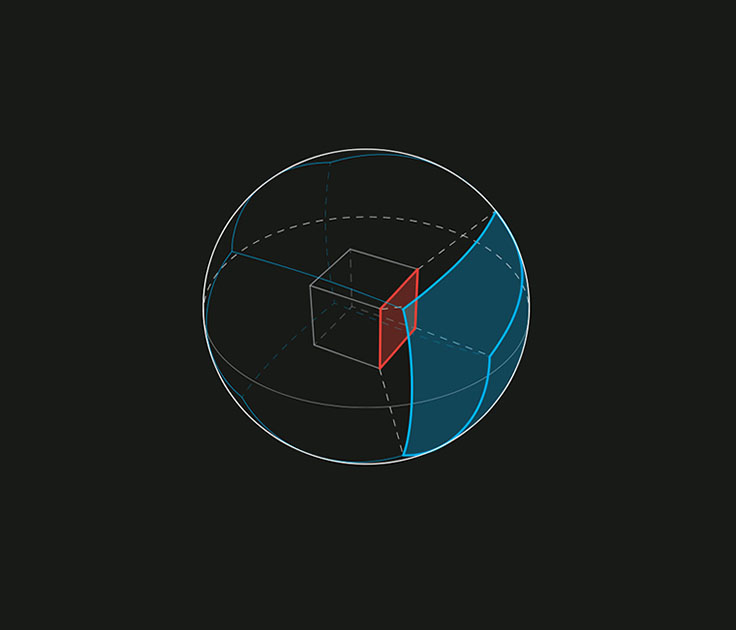
\includegraphics[width=0.8\textwidth]{figure/原理.jpg}
	\caption{360度视频原理}
	\label{fig原理}
\end{figure}
另一方面,正如\ref{fig原理}所示,用户在在观看360°视频时,用户观看的是整个球形图像的有限部分,这通常由用户的视场(FoV)(也被称为视口)决定。如果我们能够准确预测用户的运动,传输满足用户要求的视频相关部分,就能在显著降低网络带宽消耗和其他无谓的消耗,同时也保证了用户体验质量。为此,基于切片的方法被提出来用于360°视频流传输,它将每个全景帧分为较小尺寸的非重叠矩形区域,称为切片。一般来说,基于切片的流媒体利用了传输效率和用户体验之间的权衡。一方面,只有一个切片子集被传输,这可以大大减少带宽消耗;另一方面,这个子集不一定覆盖实际的用户视野,因此用户体验质量受到切片选择的极大影响。

在实践中,我们通常提供一个大于FoV的部分来容忍运动预测误差。为了让用户能够成功地查看他/她想要的内容,该部分应该成功传输并覆盖用户的视野。直观地说,传送切片部分越大,对运动预测误差的容忍度就越高,无线传输成功的几率就越低传输。传送切片部分越小,对运动预测误差的容忍度就越高,无线传输成功的几率就越低传输因此。因此我们的问题是如何在每次选择适当部分进行传输,以最大化系统吞吐量。
\label{sec:background}

\section{国内外研究现状和相关工作}
\label{sec:related_work}
近年来,已有不少针对360度视频流的传输算法研究工作。Xing Liu等\cite{ref2}提出的研究使用跨学科方法优化360°视频流。他们从系统的角度出发,使用多种方法来优化360度视频流的传输。Harsh Gupta等人\cite{ref3}考虑了一个具有两级反馈的多臂老虎机问题,将其应用于全景视频流。论文开发了KL-UCB算法的一个重要变体用来解决多臂老虎机问题。J. Chen等人\cite{ref4}考虑了全景视频流的自适应速率选择问题,并将其表述为具有两级反馈信息的多臂老虎机问题,我们提出了一种改进的Thompson采样算法,该算法有效地利用了两级反馈信息,并且证明了它的性能比单级反馈信息的性能要好得多。Tang M等人\cite{ref5}提出了一种基于时空域比特率自适应的360度视频流模型。

\section{本文的研究内容与主要工作}
我们把每个全景视频划分为一系列切片,其中每个切片具有相同持续时间的固定数量的块。在每个时隙中,可以选择块的子集进行传输。我们可以把选择不同的视频块对应为选择不同的速率,选择的切片越大,那么选择的传输速率也越大。如此,速率越大,传输成功可能性越低,但是覆盖到用户的FoV的可能性越大。
如何合理选择传输速度,使得360度视频传输系统的吞吐量最大呢?我们考虑使用强化学习的方法来解决这个问题。本文将360度全景视频速率选择问题建模为一个两级反馈的多臂老虎机问题(MAB)。MAB问题描述了一个玩家选择多个老虎机(Arm)的决策(Action)并从所选老虎机获得收益(Reward)的过程。在360度视频速率选择问题中,Arm对应不同的速率。Action是选择哪一个速率传输360度全景视频块。Reward对应传输系统的一段时间内累积吞吐量。两级反馈分别是是否覆盖到用户的FoV,是否传输成功。通过多臂老虎机的解决算法选出最合适的速度,使得累积吞吐量和最佳吞吐量之间的差距变小,即最小化遗憾(Regret)。本文进一步考虑了周期性变化的信道上传输概率发生变化的情况,提出了周期性重置Thompson Sampling算法、基于折扣窗口的Thompson Sampling算法、基于滑动窗口的Thompson Sampling算法和基于折扣滑动窗口的Thompson Sampling算法。并且通过模拟数据验证这五种算法的性能。

\section{本文的论文结构与章节安排}

\label{sec:arrangement}

本文共分为六章。第一章是绪论,描述了选题的背景和研究的意义,同时简单说明了国内外在360°视频传输的研究进展,然后说明了本文的研究内容。第二章详细描述了国内外在360°视频传输方面的相关研究,同时指出他们的研究在时变信道下的缺陷。第三章对360°视频传输建模为多臂老虎机问题并且提出基于两层反馈的汤普森采样算法进行改进来解决这个问题。第四章基于两层反馈的汤普森采样算法设计了若干算法。第五章使用模拟数据对这些算法实际效果进行测试并证明算法的有效性。第六章对全文进行总结。


